\documentclass{article}

\usepackage[french]{babel}
\usepackage[utf8]{inputenc}
\usepackage{graphicx}
\graphicspath{{figures/}}
\usepackage{amsmath, amssymb}
\usepackage[french]{varioref}
\usepackage{geometry}
\usepackage[toc, page]{appendix}
\usepackage{vmargin}
\usepackage{fancyhdr}
\pagestyle{fancy}
\usepackage{xfrac}
\usepackage{caption}
\usepackage{subcaption}

%%%%%%%%%%%%%%%% Lengths %%%%%%%%%%%%%%%%

\setmarginsrb{80pt}{60pt}{80pt}{60pt}{10pt}{10pt}{40pt}{40pt}
%% \setlength{\textwidth}{17cm}
%% \setlength{\evensidemargin}{0.2cm}
%% \setlength{\oddsidemargin}{0.2cm}

%%%%%%%%%%%%%%%% Variables %%%%%%%%%%%%%%%%
\def\projet{5}
\def\titre{Résolution approchée d'équations différentielles \rule{\linewidth}{.5pt}  Modélisation de systèmes dynamiques }
\def\groupe{1}
\def\equipe{2}

%%%%%%%%%%%%%%% Autres %%%%%%%%%%%%%%%%%%%%
\renewcommand{\headrulewidth}{1pt}
\fancyhead[L]{Algorithmique Numérique}
\fancyhead[R]{Projet n°6}

\renewcommand{\footrulewidth}{1pt}
\fancyfoot[L]{\textsc{Enseirb-Matmeca}}
\fancyfoot[C]{\thepage}
\fancyfoot[R]{\textsc{Informatique-1A}}

\begin{document}

%%%%%%%%%%%%%%%% Header %%%%%%%%%%%%%%%%
\noindent\begin{minipage}{0.98\textwidth}
  \vskip 0mm
  \noindent
  { \begin{tabular}{p{7.5cm}}
      {\bfseries \sffamily
        Projet n°\projet} \\\\ 
      {\itshape \titre}
    \end{tabular}}
  \hfill 
  \fbox{\begin{tabular}{l}
      {~\hfill \bfseries \sffamily Groupe n°\groupe\ - \'Equipe n°\equipe
        \hfill~} \\[2mm] 
      Responsable : \responsible \\
      Secrétaire : \secretary \\
      Codeurs : \others
    \end{tabular}}
  \vskip 4mm ~

  ~~~\parbox{0.95\textwidth}{\small \textit{Résumé~:} \sffamily Ce
  projet a pour but de mettre en place des méthodes résolution numériques d'équations différentielles afin de pouvoir les comparer et les appliquer sur des problèmes physiques concrets. L'intérêt réside dans le fait que ces problèmes sont régis par équation dont il existe une solution analytique, ce qui nous permettra d'évaluer l'éfficacité de nos méthodes de résolution. }
  \vskip 1mm ~
\end{minipage}

%%%%%%%%%%%%%%%% Main part %%%%%%%%%%%%%%%%
\section{Méthodes numériques de résolution d'équations différentielles}


Diverses méthodes peuvent être utilisées pour résoudre une équations différentielle, nous parlerons dans partie des équations dont les solutions peuvent être de la forme : 
\begin{center}
\fbox{$y_{n+1} = y_n + h_n\Phi(y_n, h_n, t_n)$}
\end{center}

Il existe en effet plusieurs approches permettant la résolution itératives des équations différentielles. Dans ce sens, il faudra déterminer une suite de points $(y_n, t_n)$ en prenant en compte une situation initiale $(y_0, t_0)$, et un pas $h$.


Soit le problème de Cauchy suivant : 

\[
   \left \{
   \begin{array}{r c l}
      y_0  & = & y(t_0) \\
      y'(t)  & = & f(y(t),t)\\
   \end{array}
   \right .
\]


Les $t_n$ et $y_n$ vérifient les relations suivantes:

\[
   \left \{
   \begin{array}{r c l}
      y_{n+1}  & = & hf(t_n, y_n) + y_n \\
      y(t_n)   & = & y_n \\
      t_{n+1} & = & t_n + h
   \end{array}
   \right .
\]


\subsection{Méthodes implémentées pour la résolution}


Quatres différentes méthodes de résolutions d'équations différentielles ordinaires ont été implémentées.



Nous avons tout d'abord commencé par la méthode d'\emph{EULER}.

Cette méthode d'ordre 1 est la plus simple. La méthode consiste à approcher la fonction par sa tangente au point considéré. La suite des points se calcule par récurrence à l'aide de la formule : 
\begin{center}
$y_{n+1}= y_n + hf(t_n, y_n)+ y_n$.
\end{center}


Une autre méthode permettant la prise en compte des variations entre $y_{n+1}$ et $y_n $ est la méthode du \emph{POINT MILIEU}.
Cette méthode repose sur le même principe que la méthode d'\emph{EULER}, il faut cependant déterminer le point médian entre $y_{n+1}$ et $y_n$.
Au voisinage de ce point, on approchera la solution via une parallèle à la tangente obtenu par la méthode d'\emph{EULER}.


Nous avons également implémenté la méthode de \emph{HEUN}. Cette méthode est une méthode qui suit un schéma correction-prédiction. On va utiliser  la moyenne des pentes au point initial et au point qui aurait été obtenu par la methode d'\emph{EULER} pour obtenir la position du point suivant.


Nous avons finalement implémenté la méthode de Runge-Kutta d'ordre 4 qui consiste à estimer que $y_(n+1)$ est obtenu en faisant la somme de $y_n$ et du produit de l'amplitude de l'intervalle par la pente moyenne. 


\subsection {Tests sur les différentes méthodes}


Par la suite, nous avons testé ces différentes méthodes pour savoir laquelle serait la plus efficace quant à l'approximation d'une solution à une équations donnée.

Nous avons testé ces méthodes sur le problème de cauchy suivant dont la solution exacte est $y(t) = e^{arctan(t)}$ : 

\[
   \left \{
   \begin{array}{r c l}
      y(0)  & = 1 \\
      y'(t) & = & \frac{y(t)}{1+t^2}
   \end{array}
   \right .
\]
\begin{minipage}{0.4\textwidth}
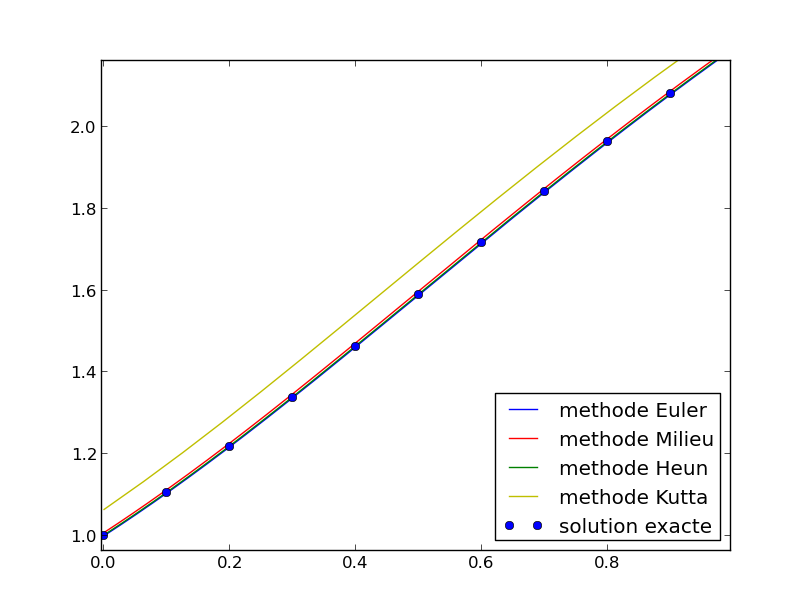
\includegraphics[scale = 0.4]{all.png}
%\captionof{solution approchée : trajectoires elliptiques}
\label{elipse}
\end{minipage} \hfill
\begin{minipage}{0.45\textwidth}
La figure ci-contre représente les résultats obtenus pour toutes les méthodes sur l'intervalle $[0,1]$. Mis à part quelques erreurs de précision dûes aux choix des pas, toutes les méthodes donnent de bonnes approximations par rapport à la solution exacte.

\end{minipage}



Ces mêmes méthodes ont été testées sur des équations à plusieurs dimensions. 
En dimension 2 par exemple où nous avons résolu le problème suivant : 
y(t) =
$\begin{pmatrix}
   y_1(t) \\
   y_2 (t) 
\end{pmatrix} $  où y'(t) = 
$\begin{pmatrix}
   -y_2(t) \\
   y_1 (t) 
\end{pmatrix}$ et y(0) =
$\begin{pmatrix}
   1 \\
   0 
\end{pmatrix} $.

\begin{minipage}{0.4\textwidth}
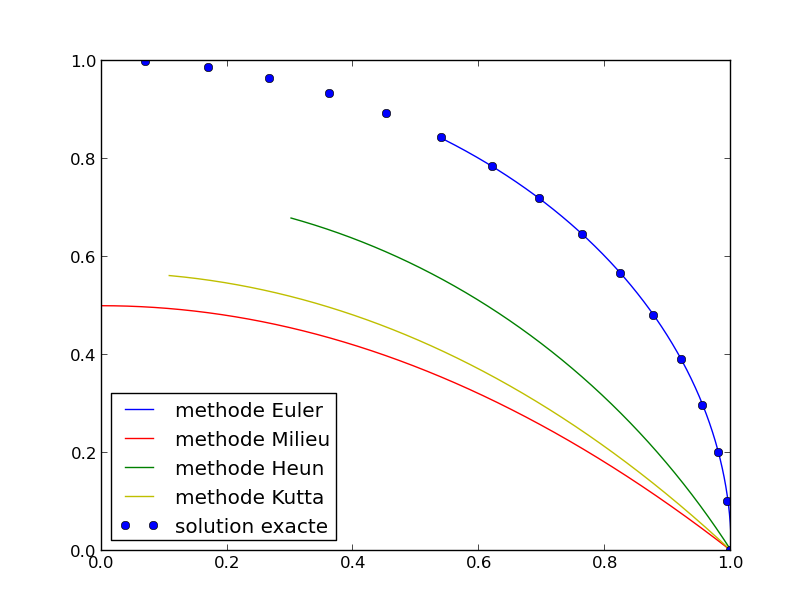
\includegraphics[scale = 0.4]{d2.png}
%\captionof{solution approchée : trajectoires elliptiques}
\label{elipse}
\end{minipage} \hfill
\begin{minipage}{0.45\textwidth}
La figure ci-contre représente les résultats obtenus pour toutes les méthodes sur l'intervalle $[0,\pi/2]$. On s'aperçoit que les erreurs d'approximation sont plus importantes dans la méthode du point milieu.
\end{minipage}

Nous remarquons que ces méthodes s'adaptent aux cas de fonctions vectorielles.
Par ailleurs nous remarquons que plus le pas est petit, plus grande est la précision.
Enfin, la méthode de Runge-Kutta apparait comme étant la méthode la plus précise, ce qui confirmé de manière analytique (méthode d'ordre 4).


\subsection{Champs des tangentes}


\begin{minipage}{0.5\textwidth}
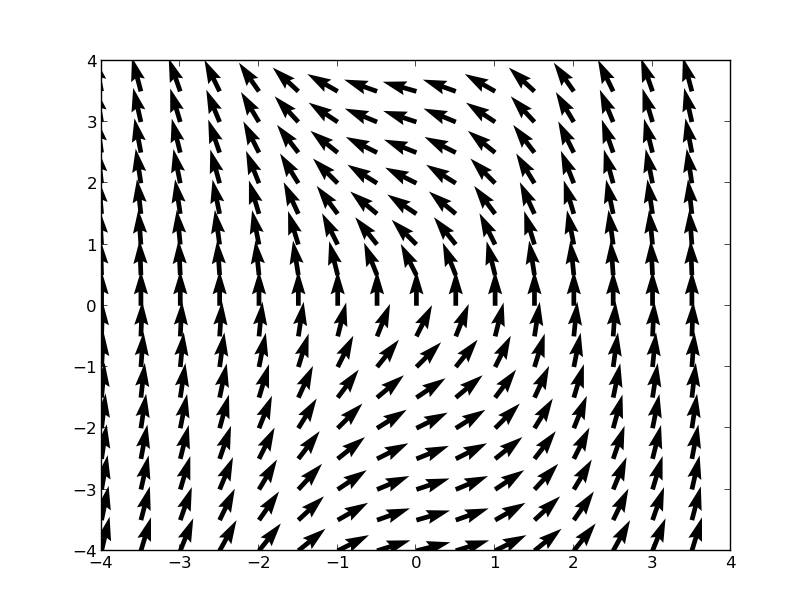
\includegraphics[scale = 0.2]{champ.jpg}
%\captionof{solution approchée : trajectoires elliptiques}
\label{elipse}
\end{minipage} \hfill
\begin{minipage}{0.5\textwidth}

Tracer le champ des tangentes déduite de $f$ nous permet d'avoir une meilleure idée de la solution. En d'autres termes il s'agit de placer un point $(x,y)$ dans le plan, pour ensuite tracer une tangente dans ce point de pente $f(x,y)$.
Pour l'équation différentielle en dimension 2  y'(t) = 
$\begin{pmatrix}
   -y_2(t) \\
   y_1 (t) 
\end{pmatrix}$ où y(0) =
$\begin{pmatrix}
   1 \\
   0 
\end{pmatrix} $ par exemple, on obtient la figure ci-contre.
Nous remarquons que le résultat que nous avons trouvé représente l'une des courbes suivies par les tangentes. 


\end{minipage}
\section{Système proie-prédateur de Lokta-Volterra}
Dans cette partie nous résolvons tous les systèmes par la méthode de Runge-Kutta exposée auparavant.

La capacité à prévoir les évolutions d'une population donnée grâce à des données environnementale a encouragé les travaux de scientifiques afin de proposer des modèles régissant ces évolutions. Les équations différentielles se revèlent être des outils fiables et pertinents pour modéliser ces variations de populations.

\subsection{Modèle de Malthus}
Malthus a proposé un modèle sur l'évolution des populations qui consiste à mesurer le taux de natalité $a$ et le taux de mortalité $b$ d'un population.

Il a établi l'équation différentielle suivante: 
\begin{equation}
\frac{\partial N(t)}{\partial t} = (a-b)N(t)
\end{equation}

On peut poser $\gamma = a-b$ qui est le taux intrinsèque d'accroissement naturel.

Les 3 types d'évolutions que l'on peut trouver dépendent du signe de $\gamma$, comme montré à la figure~\vref{fig:malthus}.

\begin{figure}
\centering
\begin{subfigure}[b]{.3\textwidth}
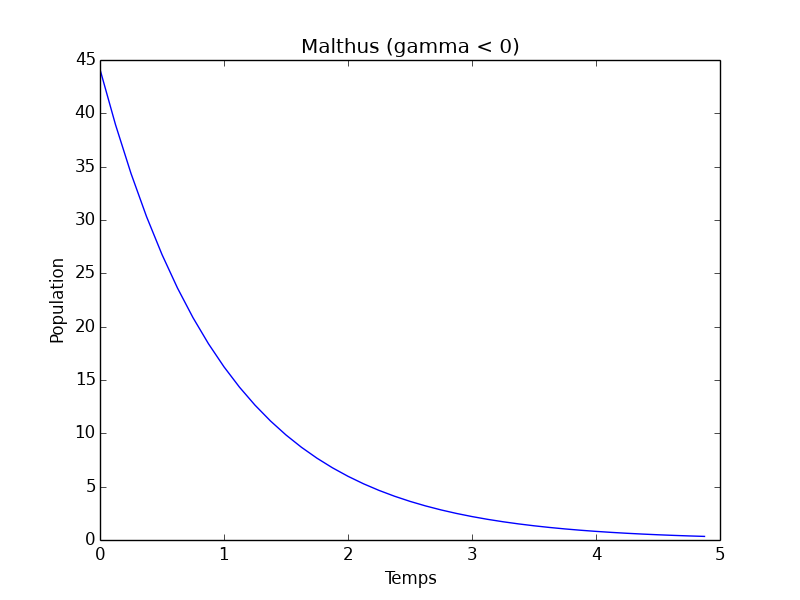
\includegraphics[width=\textwidth]{mathusinf0}
\end{subfigure}
\begin{subfigure}[b]{.3\textwidth}
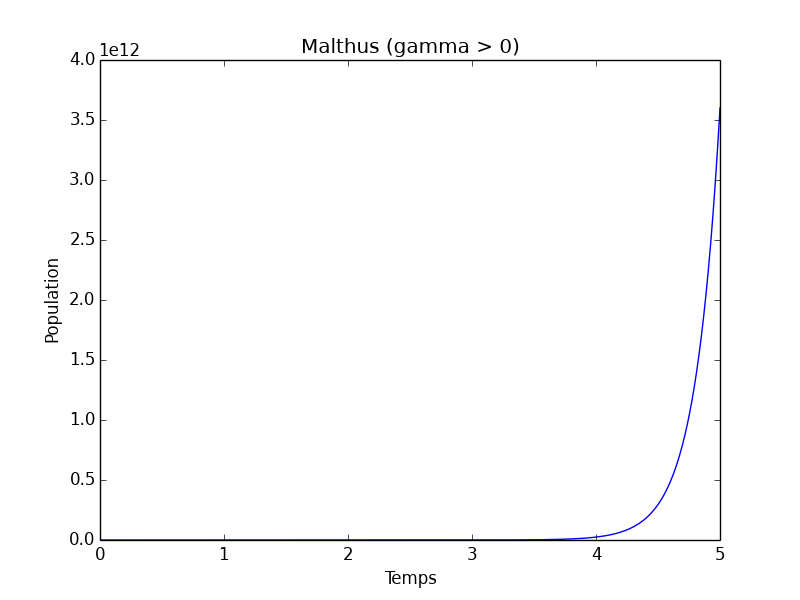
\includegraphics[width=\textwidth]{mathussup0}
\end{subfigure}

\caption{Malthus}
\label{fig:malthus}
\end{figure}

\subsection{Modèle de Verhulst}
Verhulst a proposé un modèle plus complexe pour modéliser l'évolution des populations. Dans ce modèle, il prend en compte le taux de croissance $\gamma$ et la capacité d'acceuil $\kappa$ de l'environnement.

Nous avons l'équation suivante:
\begin{equation}
\frac{\partial N(t)}{\partial t} = \gamma N(t)(1 - \frac{N(t)}{\kappa})
\end{equation}
 Ce problème peut être modélisé comme un problème de Cauchy moyennant l'ajout d'une condition initiale telle que le nombre d'invidu à t = 0.
 Cependant cette modélisation demeure simpliste de part le fait que seule la capacité d'acceuil de l'environnement soit un facteur limitant, ne tenant pas en compte l'intervention d'autres espèces. C'est pour cela que nous allons nous intéresser maintenant au système proie prédateur de Lokta-Volterra.
 
\begin{figure}
\centering
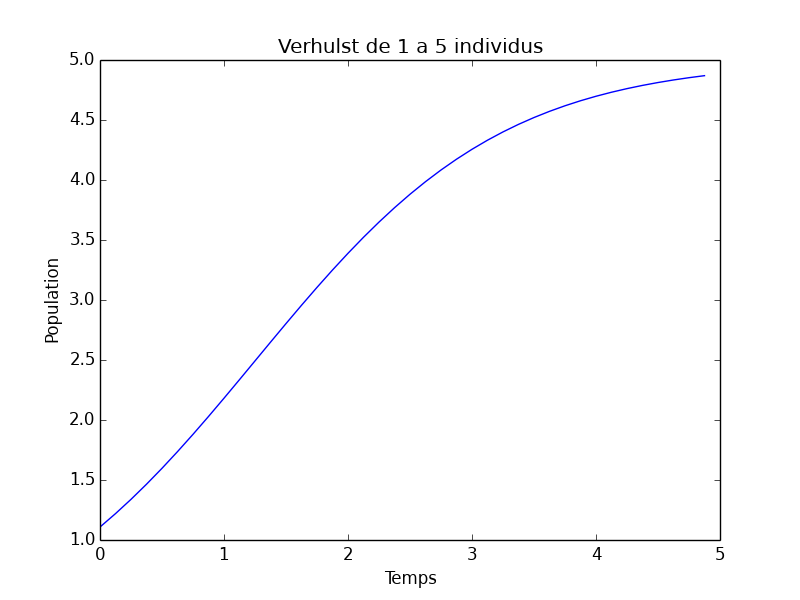
\includegraphics[width=.3\textwidth]{verhulst}

\caption{Verhulst}
\label{fig:verhulst}
\end{figure}
 
\subsection{Modèle de Lotka-Volterra}


Le modèle de population Lotka-Volterra considère l'interaction entre deux populations et nécessite deux constantes pour chaque espèce. Nous faisons l'hypothèse que les proies ne peuvent pas mourir de faim. Leur taux de mortalité est alors uniquement relié par la constante $\beta$ à la probabilité d'être mangé par un predateur, et donc au nombre de predateurs.
Une seconde constante  $\alpha$ va permettre de quantifier la rapidité de reproduction de l'espece proie, ce qui nous donne une premiere équation (3). Pour les predateurs , nous supposons que leur durée de vie est proportionnelle au nombre de leurs proies selon un coefficient  $\delta$ et nous caracterisons leur taux de mortalite par une constante $\gamma$
ce qui nous donne l'équation (4).

Nous obtenons ainsi le systeme différentiel :
\begin{equation}
\frac{\partial x(t)}{\partial t} = x(\alpha - \beta y)
\end{equation}
\begin{equation}
\frac{\partial y(t)}{\partial t} = y(\delta x - \gamma)
\end{equation}

Ce système admet une solution analytique, nous allons donc fixer des constantes pour la résoudre de manière approchée et comparer avec la solution analytique.

On peut obtenir la solution figure~\vref{fig:lv}
, avec les paramètres (1, 1, 1, 1) et la condition initiale (1.5, 1.5).

\begin{figure}
\centering
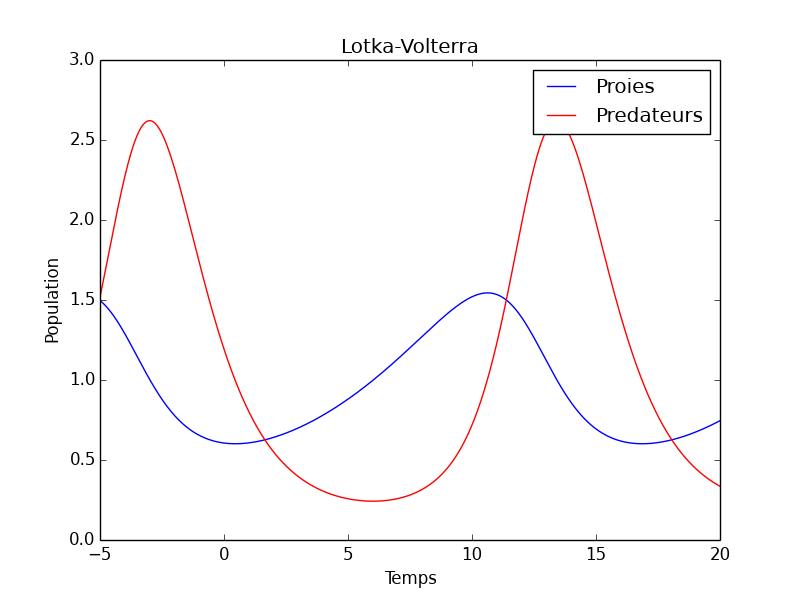
\includegraphics[width=.3\textwidth]{lotkavolterra}

\caption{Lotka-Volterra}
\label{fig:lv}
\end{figure}

La trajectoire correspondante (équation paramétrique) est tracée à la figure~\vref{fig:trajectoire}.

\begin{figure}
\centering
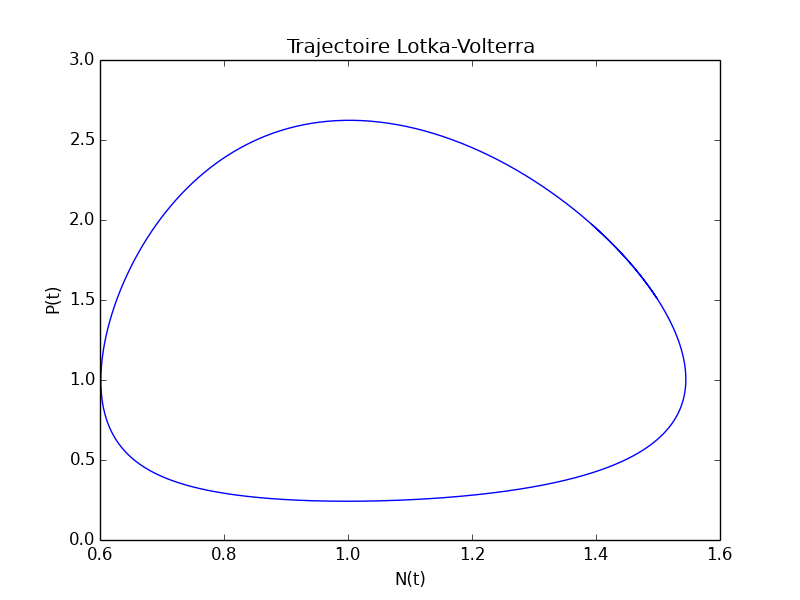
\includegraphics[width=.3\textwidth]{trajectoire}

\caption{Trajectoire}
\label{fig:trajectoire}
\end{figure}

On fait alors apparaitre des solutions périodiques, sauf dans le cas ou les deux populations sont constantes. Ces solutions correspondent aux points singuliers du systèmes : $N(t) = P(t) = 0$ ou $N(t) = \frac{d}{c}, P(t) = \frac{a}{b}$.

\begin{figure}
\centering
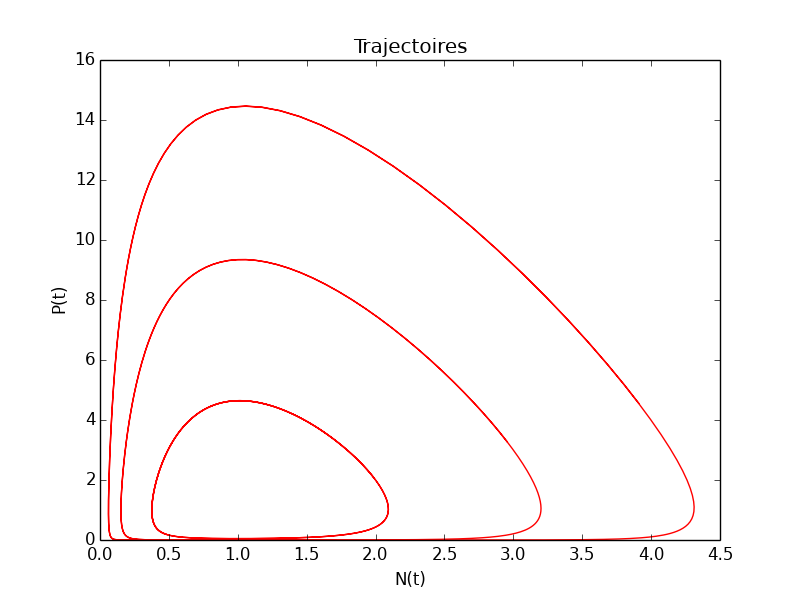
\includegraphics[width=.3\textwidth]{trajectoires}

\caption{Trajectoires}
\label{fig:trajectoires}
\end{figure}

\section{Modélisation du problème à trois corps}
Dans cette partie on s'intéresse à la résolution approchée des équations différentielles modélisants le problème à trois corps. On étudiera dans un premier temps le cas de deux astres en interaction, puis on introduira un troisième corps massif.
\subsection{Problème à deux corps}
Considérons un système composé de deux corps A et B, de masses $m_{A}$ et $m_{B}$, nous supposerons que ces deux corps sont soumis uniquement à la force gravitationnelle dûe à la présence de l'autre corps. Nous supposerons aussi que la masse de A est largement supérieure à la masse de B. Cette dernière hypothèse permet de supposer que le corps A est immobile. Nous cherchons à écrire les équations différentielles décrivants le mouvement de B dans le plan.

Pour modéliser entièrement le système nous aurons besoin de quatre inconnues représentant les coordonnées de la position et de la vitesse du corps B. Le vecteur $Y = (x_{B},y_{B},\dot x_{B},\dot y_{B})$ vérifie par application du pricipe fondamental de la dynamique l'équation différentielle suivante :

\begin{center}
$Y^{'} = f(t,Y) = \begin{pmatrix}
  \dot x_{B} \\
  \dot y_{B} \\
   \frac{Gm_{A}(x_{A} - x_{B})}{((x_{A} - x_{B})^{2} + (y_{A} - y_{B})^{2})^{\frac{3}{2}}}\\
   \frac{Gm_{A}(y_{A} - y_{B})}{((x_{A} - x_{B})^{2} + (y_{A} - y_{B})^{2})^{\frac{3}{2}}}\\
\end{pmatrix}$
\end{center}
\begin{minipage}{0.4\textwidth}
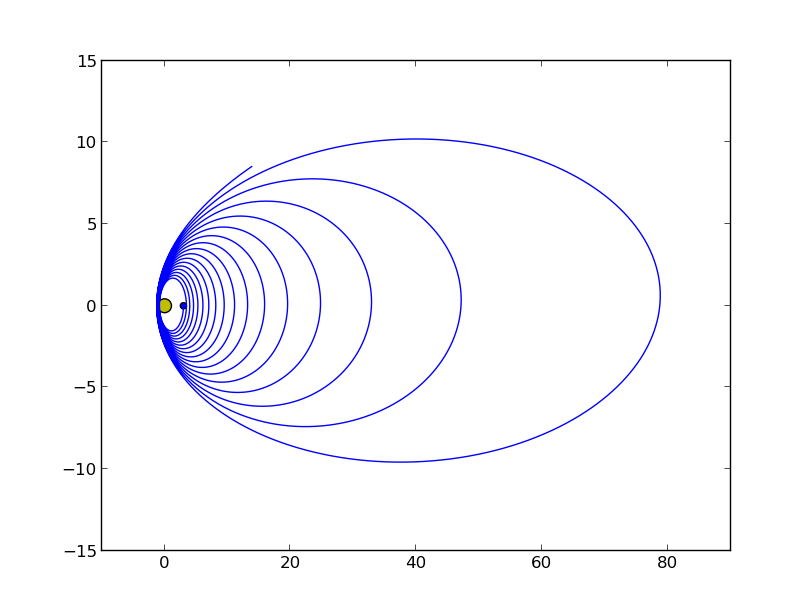
\includegraphics[scale = 0.4]{elipsoide.png}
%\captionof{solution approchée : trajectoires elliptiques}
\label{elipse}
\end{minipage} \hfill
\begin{minipage}{0.45\textwidth}
Pour obtenir une solution approchée à cette équation différentielle nous utilisons l'une des méthodes décrites dans la partie 1. La figure ~\ref{elipse} montre par exemple le résultat obtenue par la méthode d'Euler avec les conditions initales suivantes :
\begin{itemize}
\item Corps A : $(m_{A} = 100, x_{A} = 0, y_{A} = 0)$
\item Corps B : $(m_{B} = 1, x_{B} = 3, y_{B} = 0, \dot x_{B} = 0, \dot y_{B} = -3)$
\end{itemize}
En théorie, les solutions doivent correspondre à des coniques (cercles, ellipse, hyperboles et paraboles). En pratique nous n'obtenons pas de bonnes approximations pour ces coniques (ellipse dans l'exemple). En effet, plus on avance dans le temps plus ces trajectoires divergent de la conique initiale.
\end{minipage}


Ce comportement erroné est dûe à l'imprécision des méthodes de calcul, notamment le choix du pas. Nous avons remarqués dans nos test que pour toutes les méthodes, ce comportement se produit même en diminuant le pas.
\subsection{Problème à trois corps}
Nous considérons maintenant un troisième corps C de masse négligeable devant A et B. Le centre de gravité du système composé de A, B et C est situé au centre de A. De plus le corps B est supposé en rotation circulaire autour de A. Nous cherchons à obtenir la trajectoire de C.
On applique le pricipe fondamental de la dynamique à nouveau et on obtient l'équation différentielle suivante :
\begin{center}
$Y^{'} = f(t,Y) = \begin{pmatrix}
  \dot x_{C} \\
  \dot y_{C} \\
   \frac{Gm_{A}(x_{A} - x_{C})}{((x_{A} - x_{C})^{2} + (y_{A} - y_{C})^{2})^{\frac{3}{2}}} + \frac{Gm_{B}(cos(t) - x_{C})}{((cos(t) - x_{C})^{2} + (sin(t) - y_{C})^{2})^{\frac{3}{2}}}\\
   \frac{Gm_{A}(y_{A} - y_{C})}{((x_{A} - x_{C})^{2} + (y_{A} - y_{C})^{2})^{\frac{3}{2}}} + \frac{Gm_{B}(sin(t) - y_{C})}{((cos(t) - x_{C})^{2} + (sin(t) - y_{C})^{2})^{\frac{3}{2}}}\\
\end{pmatrix}$
\end{center}

Afin de bien visualer la trajectoire du point C, nous allons tracer le résultat obtenu à partir de l'une des méthodes de résolution dans le référentiel en rotation lié à B, en effectuant un changement de base. Dans ce référentiel, seul le point C est en mouvement.

La figure~\ref{cmp} représente les trajectoires de deux points C1 et C2 correspondant aux états initiaux suivants :
\begin{itemize}
\item C1 : $(x_{C1} = -0.75, y_{C1} = 0, \dot x_{C1} = 1, \dot y_{C1} = 1)$
\item C2 : $(x_{C2} = -0.7, y_{C2} = 0, \dot x_{C2} = 1, \dot y_{C2} = 1)$
\end{itemize}
On remarque que pour ces deux points dont les états initiaux sont presque confondues, les trajectoires commencent à diverger infiniment au bout d'un certain temps. On en déduit que le problème des trois corps est chaotique, c'est à dire qu'il est imprévisible et que sa solution dépend des conditions initiales.
\begin{figure}[h]
\centering
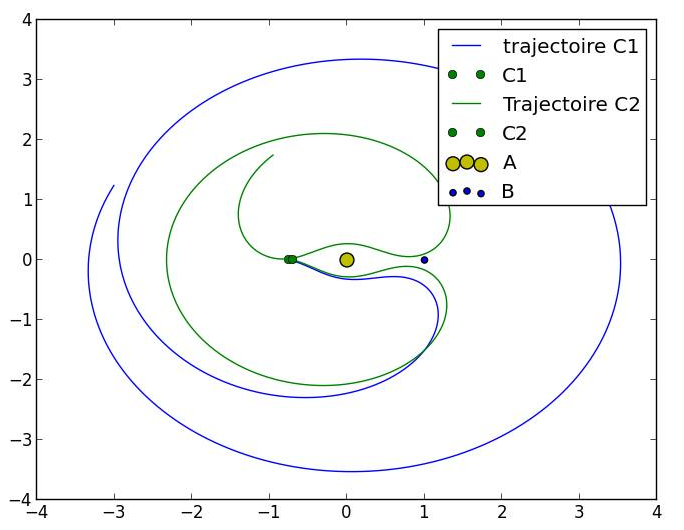
\includegraphics[scale = 0.4]{comparaison.png}
\caption{comparaison de deux trajectoires}
\label{cmp}
\end{figure}






\paragraph{Conclusion}


Plusieurs méthodes de résolutions des équations différentielles ont été implémentées durant ce projet.
Nous avons ainsi relever les différences entre les méthodes pour ensuite les tester sur des modèles physiques réalistes.
Il est à noter que la difficulté principale de ce projet est de choisir le pas qui assure une bonne précision sans entrainer un trop grand temps de calcul.
\end{document}
